\scanpage{34}
\mspage{1}
Special systems of five points on a complex sphere (more general\textsuperscript{ly} on a \deleted{\unsure{curve}} projective line over an algebraically closed field \(k\) \unsure{of characteristic \(0\)})

These are the systems \((\Sigma,K)\) with \(K\subset\Sigma\), \(\operatorname{card}K=5\), and such that there exists a nontrivial automorphism of \((\Sigma,K)\) --- that is, the group \inserted{\(G\)} of automorphisms of \((\Sigma,K)\) is not reduced to \(1\). We make the classification according to the structure of this group.

Let \(g\in G\) be of maximal order. We can identify \(g\) with a permutation of \(I\), and the discussion proceeds according to its structure. Note that \deleted{the order of \(g\ne1\) is} every automorphism of finite order of \(\Sigma\) \deleted{\(g\) of order \(5\)} has exactly two fixed points, and that \deleted{\unsure{it is}} \inserted{if the order is \(\nu\)}, \(\mathbb Z/\nu\mathbb Z\) acts freely on \(\Sigma\setminus\Sigma^g\). This shows that
\[
K=K^g\amalg\text{orbits of order }\nu,\quad\text{thus }2\leq\nu\leq5.
\]
\margin{the action is that of \(\mu_\nu\) on \(\mathbb G_m\).}

\textcircled{1} \(\nu=5\), then \(K\) is an orbit --- we may suppose that it is the orbit \(\mu_5(k)\) of \(\mu_5\) acting on \(\mathbb P^1_k\). The full group of automorphisms is \(\mathbb D_5\). Up to isomorphism, there is only one such case.

\margin{Pentagonal structure on \(I\) (``pentagon'')}
\figure{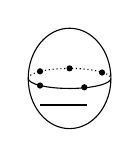
\begin{tikzpicture}[scale=.75]
\draw (0,0) ellipse(.7 and .85);
\draw (-.7,0) arc[start angle=180,end angle=360,x radius=.7,y radius=.17];
\draw[densely dotted] (-.7,0) arc[start angle=180,end angle=0,x radius=.7,y radius=.17];
\foreach \x/\y in {-.5/-.12,.25/-.15,.55/.1,-.5/.12,0/.17}{\fill(\x,\y)circle(1.5pt);}
\draw(-.5,-.45)--(.3,-.45);
\end{tikzpicture}}

\textcircled{2} \(\nu=4\) then \deleted{\(\unsure{K^g}=\operatorname{card}I^g=1\)} \inserted{\(K^g=\{P\}\)}, and \(I\setminus\{P\}\) is an orbit. We may suppose that it is \(\mu_4\), on which \(\mu_4\) acts, and \(P\) is a pole: \(\unsure{\infty}\). The full group of automorphisms is \(\mathbb Z/4\mathbb Z\simeq\mu_4(k)\).

The category of these configurations is equivalent to that of oriented squares.

\margin{``square pyramid''}
\figure{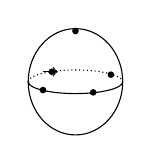
\begin{tikzpicture}[scale=.75]
\draw(0,0)ellipse(.8 and .9);
\draw(-.8,0)arc[start angle=180,end angle=360,x radius=.8,y radius=.2];
\draw[densely dotted](-.8,0)arc[start angle=180,end angle=0,x radius=.8,y radius=.2];
\foreach \x/\y in {0/.86,-.55/-.14,.3/-.18,.6/.12,-.4/.17}{\fill(\x,\y)circle(1.6pt);}
\draw[->](-.55,.17)--(-.3,.17);
\end{tikzpicture}}

\textcircled{3} \(\nu=3\), Then \deleted{\(\unsure{K}\)} \(\operatorname{card}K^g=2\), \inserted{thus \(K^g=\Sigma^g\)}, and \(I\setminus K^g\) \inserted{\(=J\)} an orbit,
\deleted{The full group of}
which we may \unsure{suppose|take} to be \(\mu_3\). The category of these configurations is equivalent to that of combinatorial triangles, that is, the one \(\mathrm{Ens}(3)\) of sets \(J\) of cardinality \(3\).

To \(J\) we associate \(\Sigma_J\deleted{\unsure{\Sigma}}\) with \(J\cup P_J\) (\(P_J\subset\Sigma_J^{\unsure{g}}\) set of the two poles of \(\Sigma_J\) \unsure{for a|in} \(1\)-\(1\) correspondence with the set \(\omega(J)\) of orientations of \(J\), if \(\unsure{k|K}=\mathbb C\)). Group of automorphisms is \(\mathbb D_3\).

\margin{\unsure{Partition} \(2\) and \(3\) (by order of \unsure{cardinalities|values} or \unsure{symmetries})}
\margin{``bitetrahedron''}
\figure{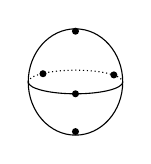
\begin{tikzpicture}[scale=.75]
\draw(0,0)ellipse(.8 and .9);
\draw(-.8,0)arc[start angle=180,end angle=360,x radius=.8,y radius=.2];
\draw[densely dotted](-.8,0)arc[start angle=180,end angle=0,x radius=.8,y radius=.2];
\foreach \x/\y in {0/.86,0/-.84,0/-.2,-.55/.14,.65/.12}{\fill(\x,\y)circle(1.7pt);}
\end{tikzpicture}}
\mspage{33}
